\documentclass[12pt,twoside]{article}
\usepackage{fancyhdr}
\usepackage{light}
\usepackage{float}
\usepackage{subfigure}
\usepackage{enumitem}
\usepackage{graphicx}
\RequirePackage{cases}


%\showsolutions
\hidesolutions

\begin{document}

\begin{problem}{20}
\textbf{Bounding sums with integrals} 
% From MCS, Problem 14.9

Assume $n$ is an integer larger than 1.  Circle all the correct inequalities below. 

Explanations are not required, but partial credit for wrong answers
will not be given without them. You may find the graphs in Figure~\ref{integrals_1overx_logx} helpful. 

\begin{figure}
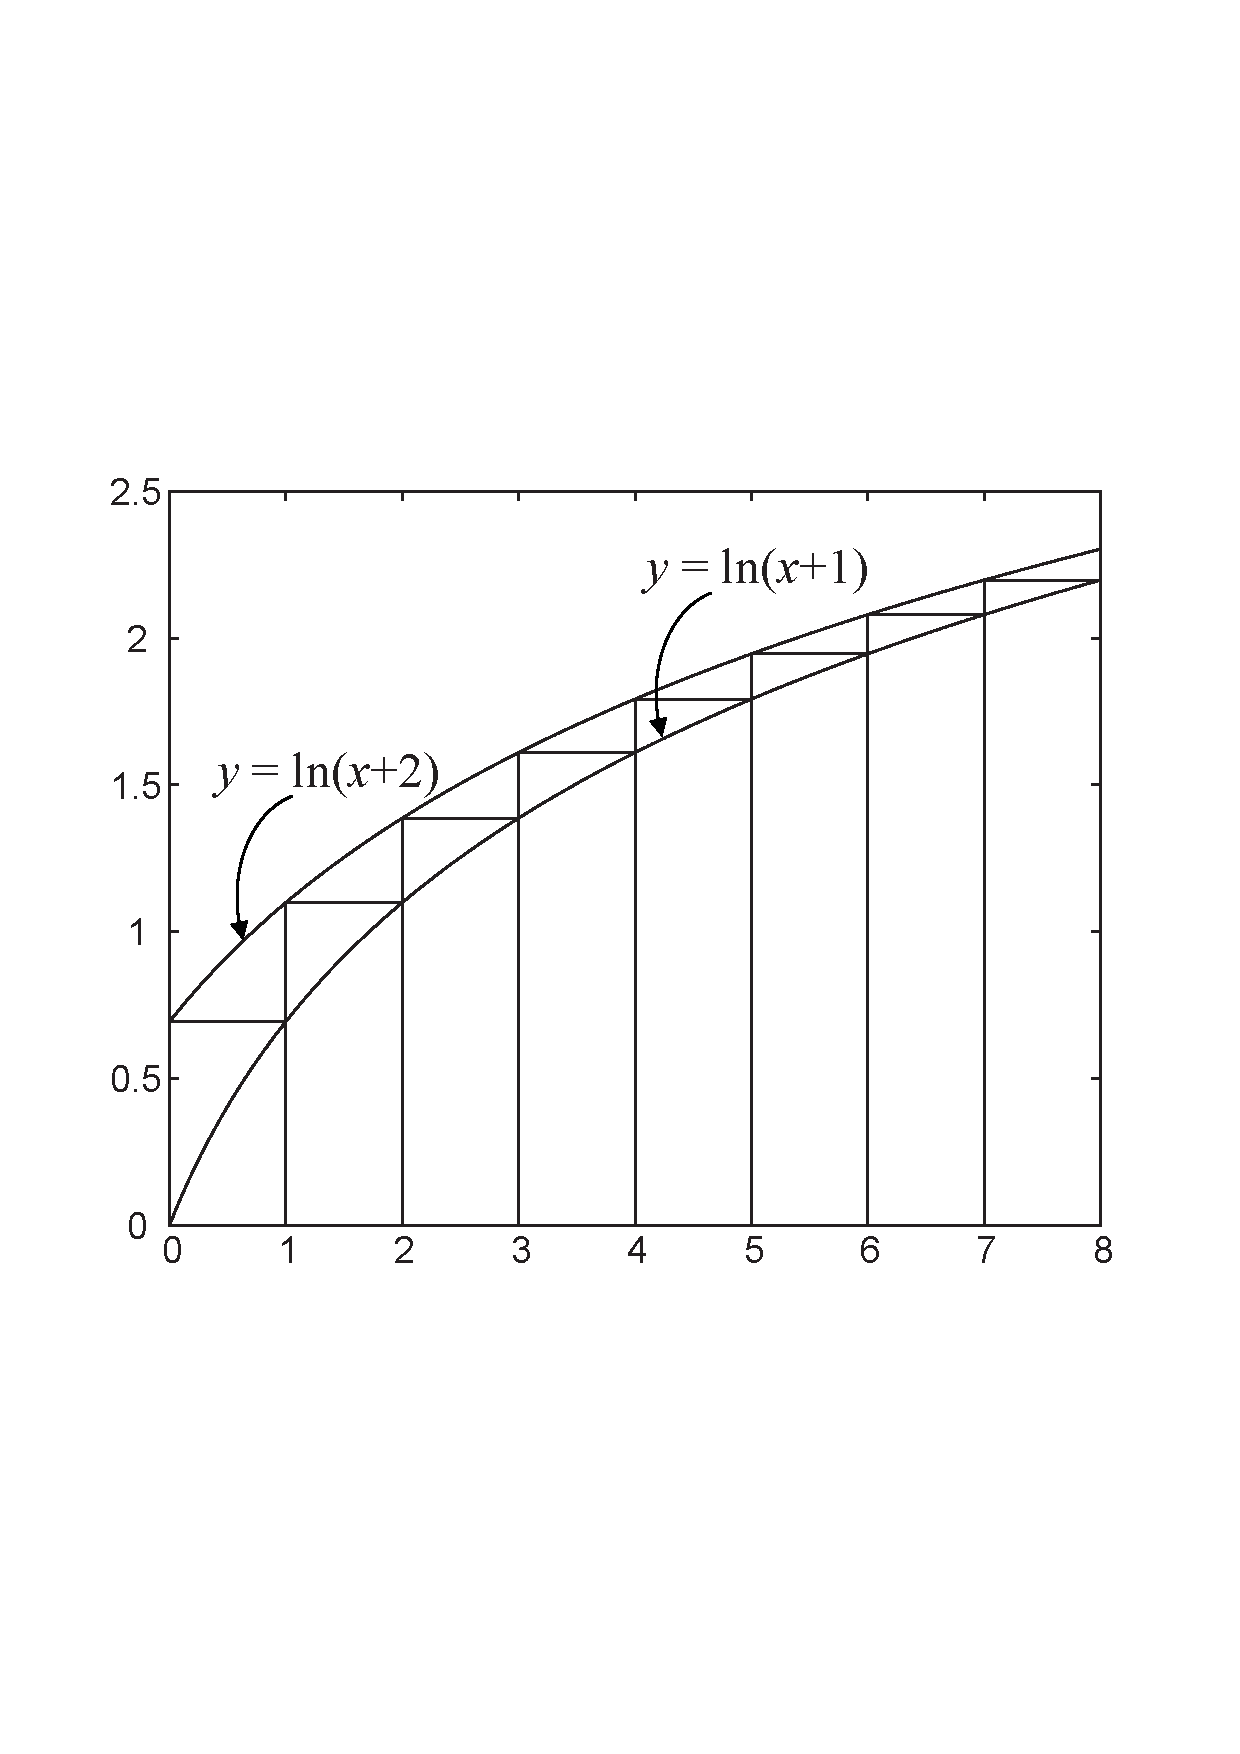
\includegraphics[width=3in,clip]{mq-integral1}
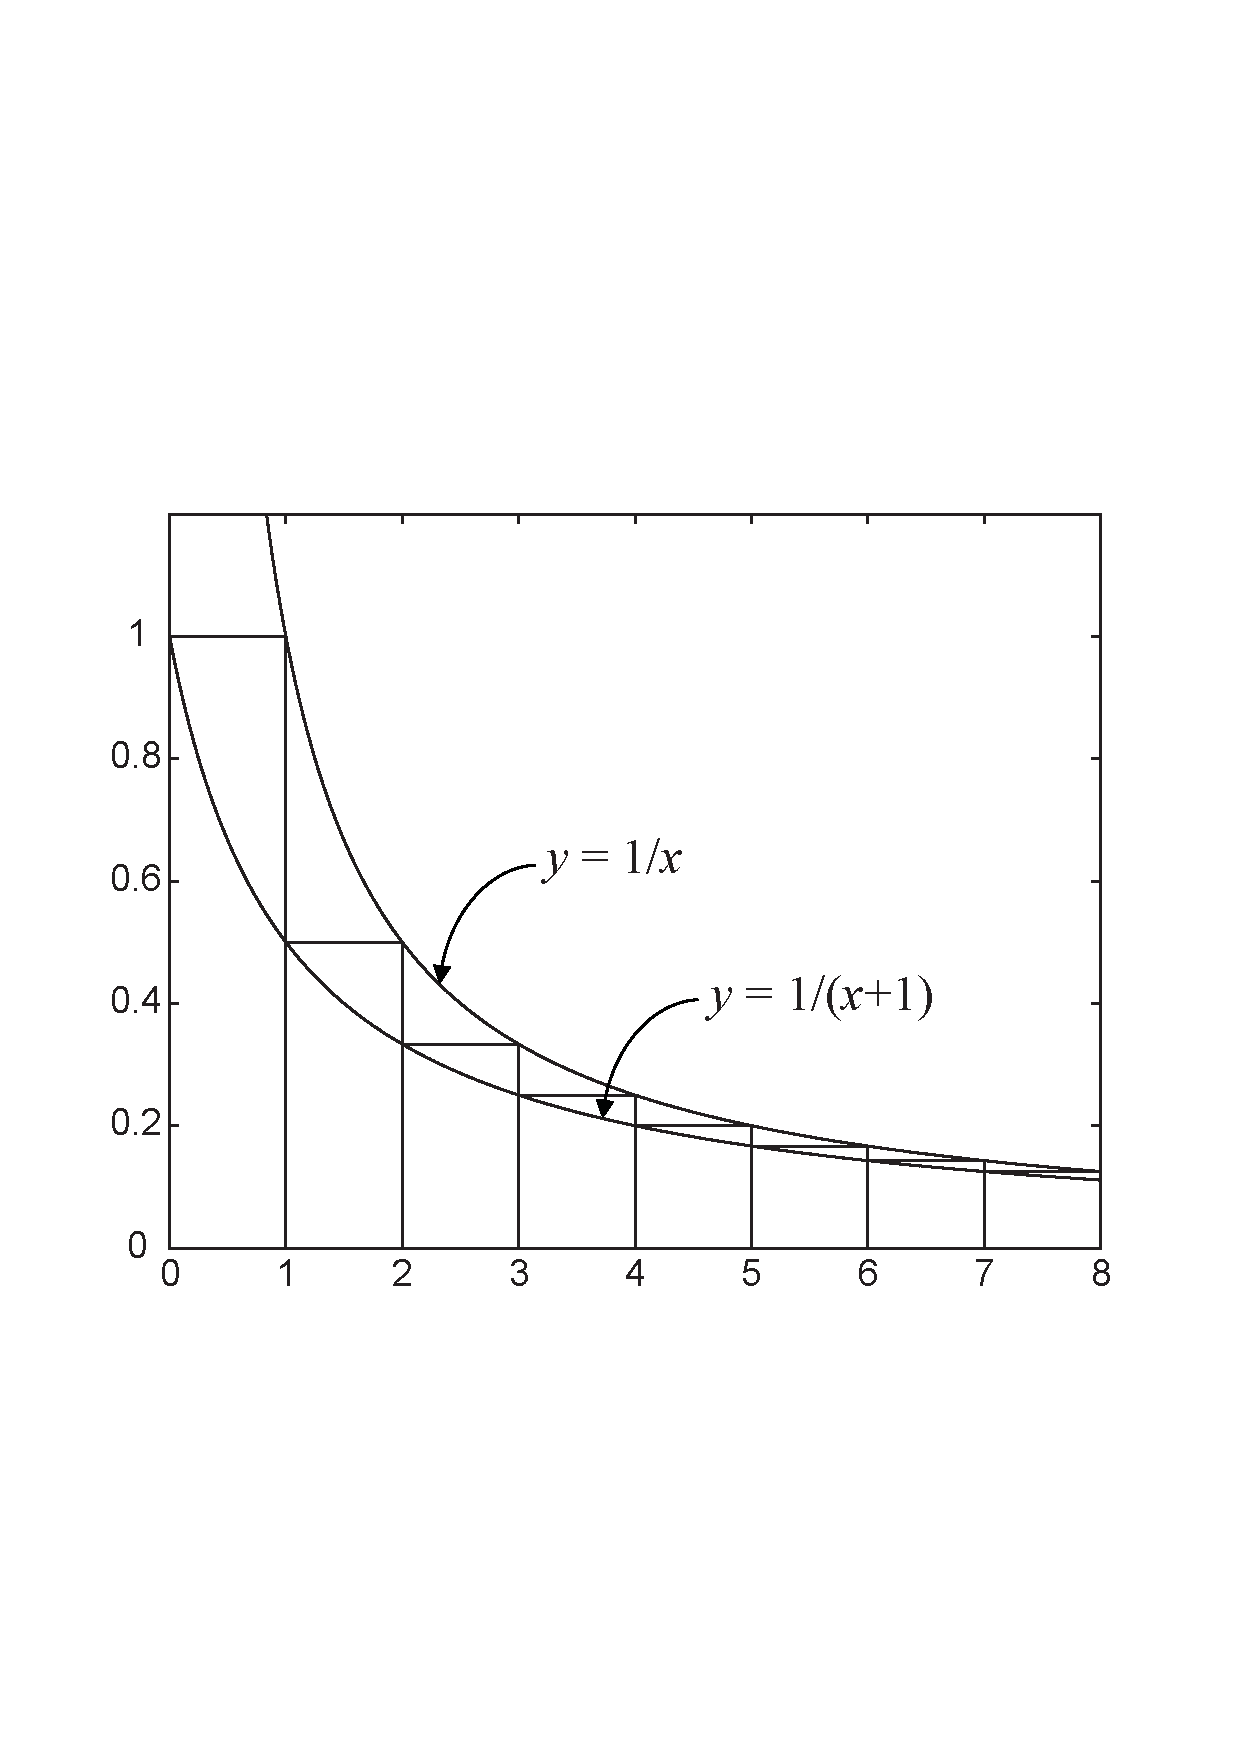
\includegraphics[width=3in,clip]{mq-integral2}
\caption{Integral bounds for two sums}
\label{integrals_1overx_logx}
\end{figure}

\begin{itemize}

\item $\displaystyle \sum_{i=1}^n \ln (i+1) \le \ln 2 + \int_1^n
\ln(x+1) dx $

\item $\displaystyle \sum_{i=1}^n \ln (i+1) \le \int_0^n \ln(x+2)
dx $

\item $\displaystyle \sum_{i=1}^n \frac{1}{i} \ge \int_0^n
\frac{1}{x+1} dx $

\item $\displaystyle \sum_{i=1}^n \frac{1}{i} \le 1.5 + \int_3^n
\frac{1}{x} dx $


\end{itemize}

\solution{The 2nd and 3rd inequalities hold.}


\end{problem}

\end{document}
